\documentclass{tietreport}

% Import images and drawing tools
\usepackage{graphicx}
\usepackage{xcolor}
\usepackage{tikz}
\usepackage{booktabs}
\usepackage{array}
\usepackage{float}
\usepackage{placeins}
\usepackage{xurl}
\usetikzlibrary{arrows.meta,positioning,shapes.geometric,fit,backgrounds}

% Bibliography configuration copied from the supplied TIET format
\usepackage[
  date=year,
  style=alphabetic,
  backend=biber,
  sorting=nty,
  maxnames=5,
  minnames=3,
  maxalphanames=4,
  minalphanames=3,
  backref=true,
  doi=false,
  isbn=false,
  url=false,
  eprint=false
]{biblatex}
\addbibresource{references.bib}
\AtEveryBibitem{\clearfield{url}\clearfield{urldate}}

\TitlePageHeader{UCS503 - Software Engineering}
\ProjectTitle{Estate Desk}
\ProjectSubTitle{A WhatsApp-Based AI Real-Estate Lead and Meeting Assistant}
\author{%
  \texttt{1024240140} Aman Kapoor \\
  \texttt{1024240020} Vidushi Jain%
}
\TitlePageSubText{Group: \texttt{3X11} BE Third Year, CSE}
\AdvisorName{}
\TitlePageFooterText{{%
    \large Project Proposal \\[0.2cm]
    \bfseries Computer Science and Engineering Department%
  } \\[0.15cm]
  Thapar Institute of Engineering and Technology, Patiala%
}

\definecolor{navy}{HTML}{17324D}
\definecolor{blue}{HTML}{3777A8}
\definecolor{teal}{HTML}{2A8C82}
\definecolor{orange}{HTML}{D97732}
\definecolor{cream}{HTML}{FFF4E8}
\definecolor{pale}{HTML}{EAF4F7}
\definecolor{green}{HTML}{DDF3E8}
\definecolor{red}{HTML}{F8DFDF}
\hypersetup{colorlinks=true,linkcolor=navy,urlcolor=blue,citecolor=teal}

\tikzset{
  flowbox/.style={draw=navy,rounded corners=3pt,thick,align=center,
    minimum height=10mm,text width=29mm,fill=pale,font=\small},
  process/.style={draw=blue,rounded corners=3pt,thick,align=center,
    minimum height=10mm,text width=31mm,fill=cream,font=\small},
  decision/.style={diamond,draw=orange,thick,aspect=2.1,align=center,
    inner sep=1pt,text width=25mm,fill=cream,font=\scriptsize},
  datastore/.style={cylinder,shape border rotate=90,draw=teal,thick,
    aspect=0.28,align=center,minimum height=12mm,text width=24mm,
    fill=green,font=\small},
  lane/.style={draw=navy!35,rounded corners=4pt,fill=#1,inner sep=7pt},
  arrow/.style={-{Latex[length=2.2mm]},thick,draw=navy},
  dashedarrow/.style={-{Latex[length=2mm]},thick,dashed,draw=teal},
  tag/.style={font=\scriptsize,fill=white,inner sep=1pt}
}

\begin{document}
\raggedbottom
\maketitle
\tableofcontents

% ===== CHAPTER 1: INTRODUCTION =====
\chapter{Introduction}

\section{Background and Context}

Property buyers already use WhatsApp to ask about price, location, bedrooms,
amenities and site visits. A small real-estate team may receive many such
conversations at the same time. Important details are spread across long chat
threads, so a manager must repeatedly read messages before deciding which buyer
needs attention. This delays replies and can cause a useful lead to be missed.

Estate Desk is proposed as a WhatsApp-first customer engagement platform. The
buyer continues to use WhatsApp, while the property manager uses a web
dashboard. A narrowly scoped OpenClaw agent answers only real-estate questions,
collects buyer requirements, recommends properties from an uploaded catalog and
asks interested buyers whether they want a physical property visit. The
dashboard turns the permitted chat into simple lead, meeting and trend views.

\subsection{Problem Statement}

The project addresses four connected problems:

\begin{itemize}
  \item buyer needs such as budget, preferred sector, bedroom count and buying
    timeline are written in different ways across many messages;
  \item managers may not know which available properties best match a buyer;
  \item interest in a physical visit may not be noticed at the right time; and
  \item normal chatbots may answer unrelated questions, invent property facts or
    mix the context of different buyers.
\end{itemize}

The proposed system must therefore be useful without becoming an uncontrolled
general-purpose assistant. It will use only authorized contacts and uploaded
property data. Prices, legal facts, availability and final meeting details will
always be checked by a human manager.

\section{Project Objectives}

\begin{enumerate}
  \item \textbf{Build a WhatsApp-first property agent:} connect one manager's
    WhatsApp account to OpenClaw and keep separate context for every buyer.
  \item \textbf{Collect structured requirements:} identify budget, BHK, area,
    property type, timeline and visit interest from normal conversation.
  \item \textbf{Recommend grounded properties:} suggest only records that exist
    in the manager's uploaded property catalog.
  \item \textbf{Give managers live guidance:} update overview, leads, meetings
    and trends pages as valid WhatsApp events arrive.
  \item \textbf{Protect scope and consent:} refuse unrelated tasks, block unknown
    contacts, obey STOP and require a human to confirm important actions.
\end{enumerate}

Figure~\ref{fig:user-journey} shows the complete user journey at a simple level.
The website is not a second chat application; it helps the manager understand
and act on the WhatsApp conversation.

\begin{figure}[H]
\centering
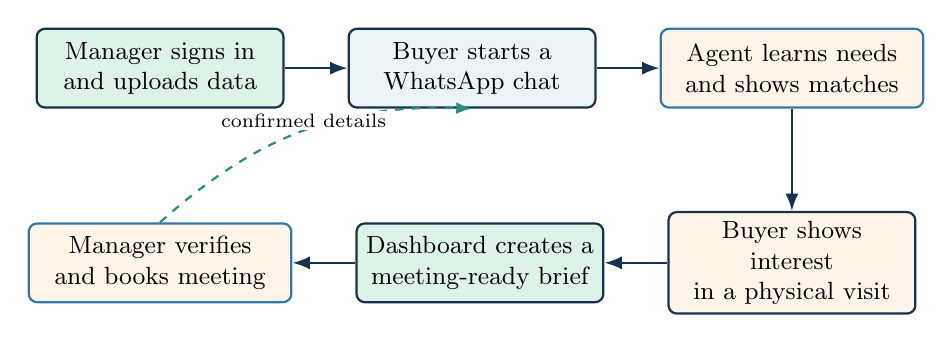
\begin{tikzpicture}[node distance=8mm and 8mm]
  \node[flowbox,fill=green] (setup) {Manager signs in\\and uploads data};
  \node[flowbox,right=of setup] (chat) {Buyer starts a\\WhatsApp chat};
  \node[process,right=of chat] (learn) {Agent learns needs\\and shows matches};
  \node[flowbox,below=13mm of learn,fill=cream] (visit) {Buyer shows interest\\in a physical visit};
  \node[flowbox,left=of visit,fill=green] (dashboard) {Dashboard creates a\\meeting-ready brief};
  \node[process,left=of dashboard] (human) {Manager verifies\\and books meeting};
  \draw[arrow] (setup) -- (chat);
  \draw[arrow] (chat) -- (learn);
  \draw[arrow] (learn) -- (visit);
  \draw[arrow] (visit) -- (dashboard);
  \draw[arrow] (dashboard) -- (human);
  \draw[dashedarrow] (human.north) to[bend left=22] node[tag,above]{confirmed details} (chat.south);
\end{tikzpicture}
\caption{Estate Desk user journey from setup to a human-confirmed visit.}
\label{fig:user-journey}
\end{figure}
\FloatBarrier

\section{Project Scope}

The prototype will support phone-number sign-up and login, CRM and listing CSV
uploads, a separate WhatsApp real-estate personality, signed message-event
ingestion, lead summaries, property matching, meeting readiness, trend analysis
and CSV exports. The supplied historical Gurgaon listings are sample data and
must not be presented as live offers.

Direct contracts with commercial CRM vendors, payment collection, legal advice,
property ownership verification and automatic meeting confirmation are outside
the first version. These limits keep the student project practical and make its
safety rules clear.

% ===== CHAPTER 2: METHODOLOGY & DESIGN =====
\chapter{Methodology and Design}

\section{System Architecture}

The system uses two connected parts. OpenClaw runs the WhatsApp channel and the
real-estate agent. Estate Desk stores workspace data and shows results to the
manager. A signed event hook sends successful incoming and outgoing message
events from OpenClaw to the web application. This separation makes it possible
to change the model or dashboard without rebuilding the complete system.

\subsection{High-Level Design}

Figure~\ref{fig:architecture} uses layers to show where each responsibility
belongs. Contact authorization and the real-estate-only policy are applied
before an answer is sent. The web application validates every event again before
it updates the database or manager screens.

\begin{figure}[H]
\centering
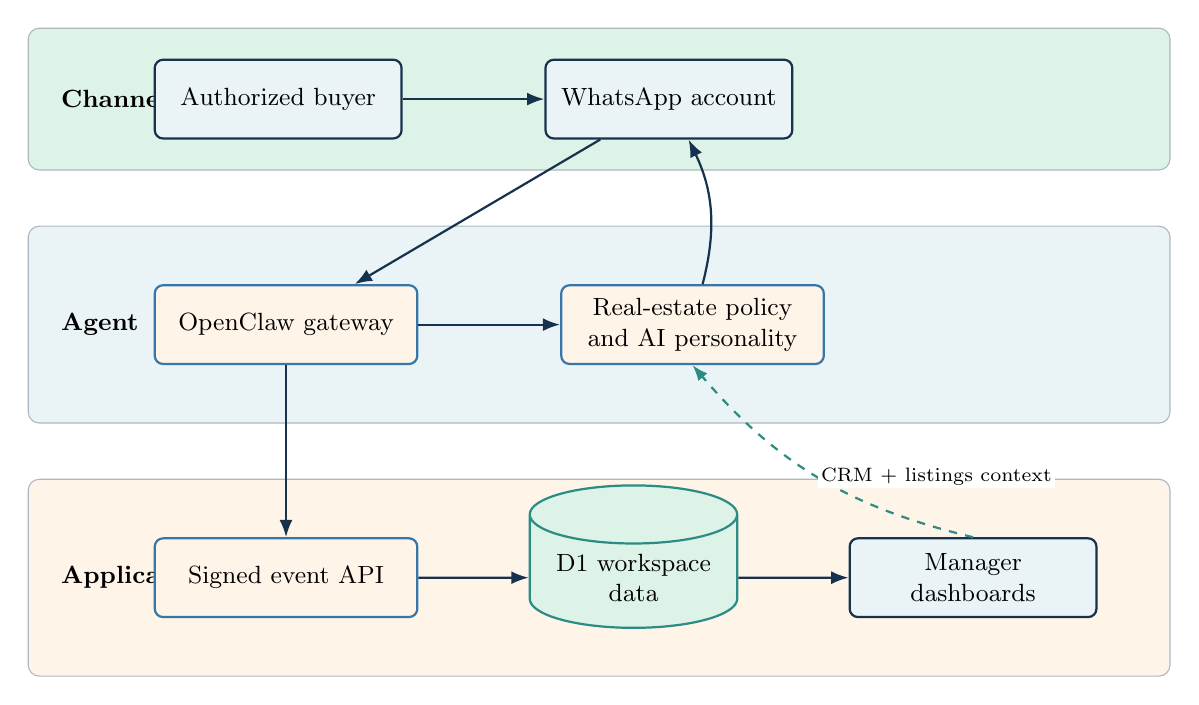
\begin{tikzpicture}[node distance=8mm]
  \node[lane=green,minimum width=145mm,minimum height=18mm] (channel) {};
  \node[font=\bfseries\small,anchor=west] at ([xshift=3mm]channel.west) {Channel};
  \node[flowbox,right=16mm of channel.west,anchor=west] (buyer) {Authorized buyer};
  \node[flowbox,right=18mm of buyer] (wa) {WhatsApp account};
  \node[lane=pale,below=7mm of channel,minimum width=145mm,minimum height=25mm] (agentlane) {};
  \node[font=\bfseries\small,anchor=west] at ([xshift=3mm]agentlane.west) {Agent};
  \node[process,right=16mm of agentlane.west,anchor=west] (gateway) {OpenClaw gateway};
  \node[process,right=18mm of gateway] (policy) {Real-estate policy\\and AI personality};
  \node[lane=cream,below=7mm of agentlane,minimum width=145mm,minimum height=25mm] (applane) {};
  \node[font=\bfseries\small,anchor=west] at ([xshift=3mm]applane.west) {Application};
  \node[process,right=16mm of applane.west,anchor=west] (api) {Signed event API};
  \node[datastore,right=14mm of api] (db) {D1 workspace\\data};
  \node[flowbox,right=14mm of db] (dash) {Manager dashboards};
  \draw[arrow] (buyer) -- (wa);
  \draw[arrow] (wa) -- (gateway);
  \draw[arrow] (gateway) -- (policy);
  \draw[arrow] (policy) to[bend right=20] (wa);
  \draw[arrow] (gateway) -- (api);
  \draw[arrow] (api) -- (db);
  \draw[arrow] (db) -- (dash);
  \draw[dashedarrow] (dash.north) to[bend left=18] node[tag,right]{CRM + listings context} (policy.south);
\end{tikzpicture}
\caption{Layered architecture for the WhatsApp agent and manager dashboard.}
\label{fig:architecture}
\end{figure}
\FloatBarrier

\subsection{Technical Stack}

\begin{itemize}
  \item \textbf{Framework and language:} Vinext/React with TypeScript for the
    web interface and server routes.
  \item \textbf{Database:} Cloudflare D1 for workspaces, contacts, listings,
    message events, buyer facts and property matches.
  \item \textbf{AI and messaging:} OpenClaw for WhatsApp routing and a separate
    real-estate agent identity with per-contact sessions.
  \item \textbf{Live updates:} server-sent events so open dashboards refresh
    after a valid message is processed.
  \item \textbf{Data exchange:} CSV upload and export for the prototype CRM and
    property catalog.
  \item \textbf{Testing and version control:} TypeScript checks, domain tests,
    API smoke tests, production builds and GitHub.
\end{itemize}

The design uses familiar and mature web tools, so the team can focus on workflow,
safety rules and evaluation. Cloudflare D1 provides an SQL model that fits
contacts, listings and message events \cite{cloudflared1}. WhatsApp business
messaging requires clear user choice and responsible handling
\cite{whatsapppolicy}.

\section{Implementation Details}

\subsection{Module 1: Onboarding and Workspace Data}

The landing page asks the manager to sign up or log in with a phone number. A
new workspace cannot open the full dashboard until the manager supplies two
datasets. The CRM CSV contains authorized client phone numbers and consent
states. The listing CSV contains property ID, location, price, BHK, area,
property type and availability notes. Managers may also add a client or property
through a form. Each workspace is kept separate from every other workspace.

The prototype provides downloadable templates and a normalized sample catalog
from a historical Gurgaon dataset. Import checks reject missing columns, invalid
phone numbers and badly formed price values. Duplicate contacts and listing IDs
are updated carefully instead of being copied many times.

\subsection{Module 2: WhatsApp Event and Insight Pipeline}

Each received or successfully sent WhatsApp message gets a unique event ID. The
hook includes the account, channel, contact, direction, time and message text in
a signed request. The API checks the signature, workspace, contact, channel,
event size and ID. Repeated IDs are ignored. This gives the dashboard a clean
event ledger and avoids counting one message twice.

After a valid event is stored, the analysis service updates the buyer profile,
lead stage and property ranking. Figure~\ref{fig:realtime} is a sequence-style
flowchart: time moves from left to right, while each vertical line represents a
different part of the system.

\begin{figure}[H]
\centering
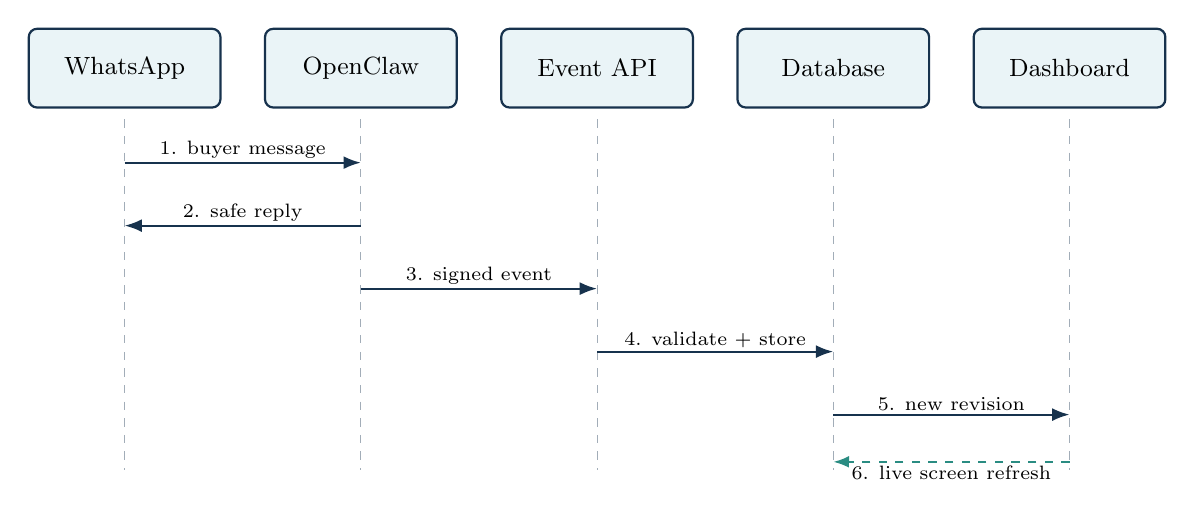
\begin{tikzpicture}[x=1cm,y=1cm]
  \foreach \x/\name in {0/WhatsApp,3/OpenClaw,6/Event API,9/Database,12/Dashboard}{
    \node[flowbox,text width=22mm] (h\x) at (\x,0) {\name};
    \draw[navy!40,dashed] (\x,-0.65) -- (\x,-5.1);
  }
  \draw[arrow] (0,-1.2) -- node[tag,above]{1. buyer message} (3,-1.2);
  \draw[arrow] (3,-2.0) -- node[tag,above]{2. safe reply} (0,-2.0);
  \draw[arrow] (3,-2.8) -- node[tag,above]{3. signed event} (6,-2.8);
  \draw[arrow] (6,-3.6) -- node[tag,above]{4. validate + store} (9,-3.6);
  \draw[arrow] (9,-4.4) -- node[tag,above]{5. new revision} (12,-4.4);
  \draw[dashedarrow] (12,-5.0) -- node[tag,below]{6. live screen refresh} (9,-5.0);
\end{tikzpicture}
\caption{Near-real-time message sequence from WhatsApp to the dashboard.}
\label{fig:realtime}
\end{figure}
\FloatBarrier

\subsection{Module 3: Real-Estate Agent and Safety Rules}

The agent asks one or two useful questions at a time and keeps a separate
conversation for each contact. Its goal is to understand the buyer and, when
there is enough interest, ask whether the buyer wants a physical visit at one or
more matching properties. It must never invent a listing, promise availability,
confirm a booking or discuss unrelated topics.

Safety does not depend only on the personality prompt. A second policy layer
checks the channel, recipient, consent state and outgoing content. Unknown
contacts are blocked. An inbound-only contact may receive replies but no cold
outreach. STOP changes the contact to opted-out immediately. Suspicious requests
receive a short real-estate scope reminder. This layered approach follows the
general idea that prompt-injection risk should be handled with validation,
least privilege and clear boundaries~\cite{owaspllm}.

\subsection{Module 4: Manager Dashboards}

The \textbf{Overview} page shows lead counts, conversation activity and stage
distribution. The \textbf{Leads} page lists buyer details, known requirements,
matched properties and the recommended next action. The \textbf{Meetings} page
shows ``buyer ready for physical meeting'' cards with the buyer's contact,
requirements, useful chat facts and one or more properties to visit. The
\textbf{Trends} page compares chat demand with the listing database to show the
most requested sectors, BHK values and specific properties. A CSV export combines
agent analysis and permitted conversation data for manager use.

% ===== CHAPTER 3: RESULTS & EVALUATION =====
\chapter{Results and Evaluation}

\section{Testing Methodology}

This is a project proposal, so the following tests describe how the prototype
will be evaluated rather than claiming final production results.

\begin{itemize}
  \item \textbf{Unit Testing:} test phone normalization, CSV validation,
    requirement extraction, consent changes and property scoring separately.
  \item \textbf{Integration Testing:} send signed sample WhatsApp events and
    confirm that messages, lead facts, matches and live screens update together.
  \item \textbf{Performance Testing:} compare event timestamps with dashboard
    revision timestamps and measure the delay under a small pilot load.
  \item \textbf{Safety Testing:} try unrelated questions, prompt-injection text,
    unknown recipients, duplicate events and STOP/START messages.
  \item \textbf{User Testing:} ask 5--10 consenting friends or family members to
    act as buyers and ask a manager whether the resulting brief is useful.
\end{itemize}

\section{Performance Metrics}

\begin{table}[H]
\centering
\small
\begin{tabular}{>{\raggedright\arraybackslash}p{0.30\textwidth}
                >{\raggedright\arraybackslash}p{0.20\textwidth}
                >{\raggedright\arraybackslash}p{0.34\textwidth}}
\toprule
\textbf{Metric} & \textbf{Pilot target} & \textbf{How it will be measured} \\
\midrule
Valid event capture & At least 95\% & Compare test WhatsApp events with the stored event ledger \\
Useful requirement summary & At least 80\% accepted & Manager checks budget, BHK, area and timeline \\
Property grounding & 100\% catalog IDs & Compare every suggestion with the uploaded listings \\
Dashboard update delay & Under 5 seconds & Compare event and screen revision timestamps \\
STOP compliance & 100\% & Automated consent tests and manual pilot checks \\
Meeting brief usefulness & At least 80\% accepted & Manager rates whether the brief supports a real visit \\
\bottomrule
\end{tabular}
\caption{Planned performance and safety measures for the pilot.}
\label{tab:performance}
\end{table}

\section{Analysis}

The main success measure is \textbf{time to a useful manager action}: the time
between a buyer's first valid WhatsApp message and a dashboard result that tells
the manager what to ask, what properties to show or whether to arrange a visit.
The project will not use message count alone as a success measure because a long
conversation can still be unhelpful.

Figure~\ref{fig:meeting-decision} shows the rule for producing a meeting-ready
lead. The AI may detect and record interest, but the final booking stays with the
manager. This prevents a buyer from receiving a false promise about availability
or timing.

\begin{figure}[H]
\centering
\resizebox{0.96\textwidth}{!}{%
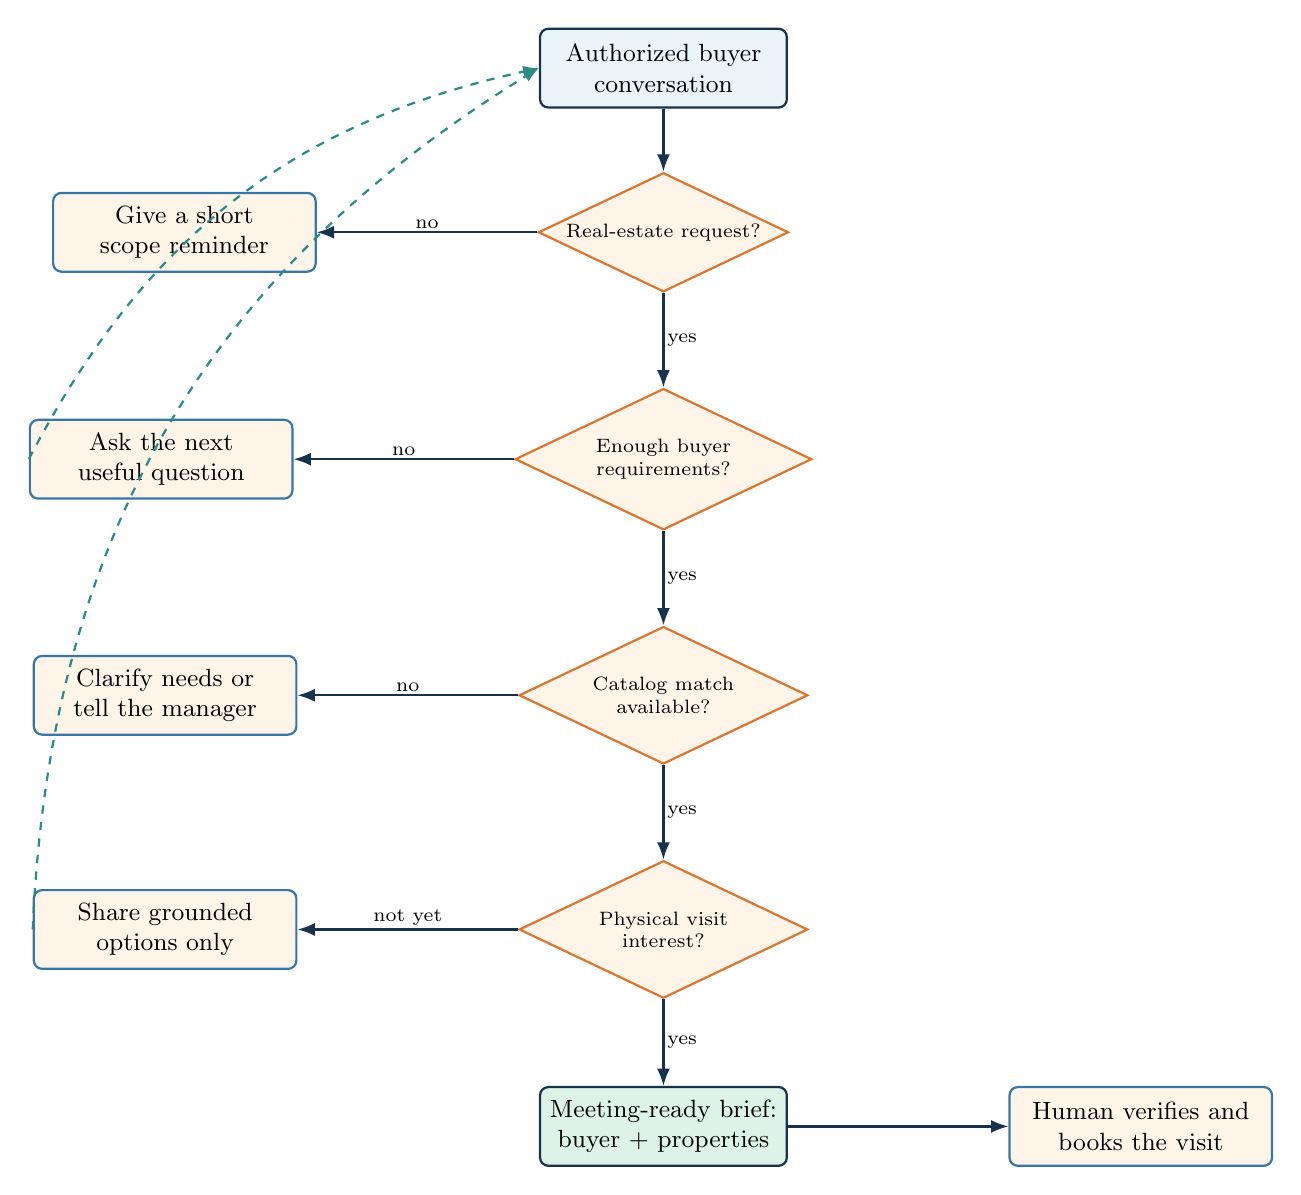
\begin{tikzpicture}[node distance=8mm and 18mm]
  \node[flowbox] (start) {Authorized buyer\\conversation};
  \node[decision,below=of start] (scope) {Real-estate request?};
  \node[process,left=28mm of scope] (limit) {Give a short\\scope reminder};
  \node[decision,below=12mm of scope] (facts) {Enough buyer\\requirements?};
  \node[process,left=28mm of facts] (ask) {Ask the next\\useful question};
  \node[decision,below=12mm of facts] (match) {Catalog match\\available?};
  \node[process,left=28mm of match] (clarify) {Clarify needs or\\tell the manager};
  \node[decision,below=12mm of match] (interest) {Physical visit\\interest?};
  \node[process,left=28mm of interest] (nurture) {Share grounded\\options only};
  \node[flowbox,below=11mm of interest,fill=green] (ready) {Meeting-ready brief:\\buyer + properties};
  \node[process,right=28mm of ready] (human) {Human verifies and\\books the visit};
  \draw[arrow] (start) -- (scope);
  \draw[arrow] (scope) -- node[tag,above]{no} (limit);
  \draw[arrow] (scope) -- node[tag,right]{yes} (facts);
  \draw[arrow] (facts) -- node[tag,above]{no} (ask);
  \draw[arrow] (facts) -- node[tag,right]{yes} (match);
  \draw[arrow] (match) -- node[tag,above]{no} (clarify);
  \draw[arrow] (match) -- node[tag,right]{yes} (interest);
  \draw[arrow] (interest) -- node[tag,above]{not yet} (nurture);
  \draw[arrow] (interest) -- node[tag,right]{yes} (ready);
  \draw[arrow] (ready) -- (human);
  \draw[dashedarrow] (ask.west) to[bend left=25] (start.west);
  \draw[dashedarrow] (nurture.west) to[bend left=28] (start.west);
\end{tikzpicture}
}
\caption{Decision flow for creating a physical-meeting-ready buyer brief.}
\label{fig:meeting-decision}
\end{figure}
\FloatBarrier

The pilot results will be reviewed in three groups. First, technical results will
show whether events arrive once and screens update quickly. Second, quality
results will show whether buyer facts and suggested listings are correct. Third,
safety results will show whether the system stays inside real estate, respects
consent and leaves important commitments to a human.

% ===== CHAPTER 4: CONCLUSION =====
\chapter{Conclusion}

\section{Summary of Work}

Estate Desk proposes a practical bridge between WhatsApp property conversations
and manager action. It combines a restricted OpenClaw real-estate agent, an
authorized CRM list, a property catalog, signed event handling and live web
dashboards. The expected result is a short, useful buyer brief that tells the
manager what the buyer wants, which uploaded properties fit and whether the
buyer appears ready for a physical meeting.

\section{Key Findings}

\begin{itemize}
  \item \textbf{The manager dashboard should support the conversation, not
    replace it.} Buyers can continue to use the familiar WhatsApp channel.
  \item \textbf{A useful lead needs both chat and listing context.} Chat alone
    cannot prove that a suitable property is actually in the manager's catalog.
  \item \textbf{Meeting readiness is an AI suggestion, not a confirmed booking.}
    A human must verify the property, time and buyer's final agreement.
  \item \textbf{Safety needs more than a prompt.} Contact authorization, consent,
    signed events and outgoing-message checks reduce avoidable misuse.
\end{itemize}

\section{Future Work and Recommendations}

\begin{enumerate}
  \item connect a real CRM through its authorized API instead of CSV files;
  \item add hosted WhatsApp connection management for multiple property teams;
  \item add staff roles, lead assignment and calendar-based meeting requests;
  \item connect verified live inventory and mark changed prices or availability;
  \item evaluate extraction and matching on a larger, consented conversation set;
  \item add stronger audit reports, retention controls and deletion tools; and
  \item compare different approved models without changing the safety boundary.
\end{enumerate}

\section{Final Remarks}

The project is suitable for a third-year software engineering team because it
has a clear user problem, separate modules, measurable targets and visible
safety limits. It also has a useful first version that can be tested with a small
group before larger integrations are attempted. The main idea is simple: let the
AI organize and qualify property interest, but let people control consent,
property truth and the final physical meeting.

\printbibliography[heading=bibintoc]
\end{document}
